Les fichiers de forçage jouent un rôle essentiel dans la modélisation océanographique. Ils fournissent au modèle les conditions aux limites et les forçages externes nécessaires pour simuler correctement les dynamiques océaniques. Dans le contexte du modèle CROCO, ces fichiers de forçage sont particulièrement cruciaux pour la simulation des mouvements induits par la marée.

\subsubsection{Rôle et importance des fichiers de forçage}

Un fichier de forçage est, en essence, un ensemble de données qui impose certaines conditions au modèle. Pour le modèle CROCO, ces conditions peuvent inclure des variations de la température de surface, de la salinité, des vents, et surtout, des forces générées par la marée. Ces données, structurées sous format netCDF, permettent au modèle de simuler les mouvements océaniques avec une précision accrue, en tenant compte des influences externes.

\subsubsection{Origine des données de forçage : les harmoniques}

Les données de forçage liées à la marée sont généralement obtenues à partir d'harmoniques. Les harmoniques de marée sont des composantes sinusoïdales qui décrivent les mouvements périodiques de la marée en fonction du temps. Chaque harmonique représente une composante spécifique de la force de marée, comme l'influence du soleil, de la lune, ou d'autres corps célestes. En combinant ces harmoniques, il est possible de reconstruire le signal de marée complet et de prévoir ses variations avec une grande précision comme expliqué dans la figure \ref{fig:harmoniques}.

Dans la section suivante, nous nous concentrerons sur le modèle de marées TPXO9, largement reconnu pour sa précision et sa fiabilité. Ce modèle, choisi pour la génération de nos fichiers de forçage, offre une représentation détaillée des mouvements de marée à l'échelle mondiale.

\subsubsection{Le modèle TPXO9}

Le modèle \href{https://www.tpxo.net/global/tpxo9-atlas}{TPXO9} est l'une des versions les plus récentes et les plus précises des modèles de marées globales développés par le groupe de recherche de l'Université de l'État de l'Ohio \cite{egbert2002efficient, erofeeva2010high}. Il s'agit d'un modèle d'altimétrie satellitaire basé sur une combinaison de données de plusieurs missions altimétriques, couvrant plusieurs décennies d'observations \cite{ray2012tide}. 

Caractéristiques clés du modèle TPXO9 :
\begin{itemize}
	\item \textbf{Résolution spatiale} : Le modèle offre une résolution de 1/30°, permettant de capturer des détails fins des mouvements de marée, y compris dans des régions complexes comme les archipels et les zones côtières.
	\item \textbf{Harmoniques} : Le modèle TPXO9 utilise un total de 13 harmoniques pour représenter les principales composantes de la marée. Ces harmoniques sont essentielles pour capturer la dynamique complexe des marées à travers le monde. Les harmoniques utilisées par TPXO9 sont les suivantes:
	
	\begin{itemize}
		\item \textbf{mm}
		\item \textbf{mf}
		\item \textbf{q1}
		\item \textbf{o1}
		\item \textbf{p1}
		\item \textbf{k1}
		\item \textbf{n2}
		\item \textbf{m2}
		\item \textbf{s2}
		\item \textbf{k2}
		\item \textbf{mn4}
		\item \textbf{m4}
		\item \textbf{ms4}
	\end{itemize}
	Chacune de ces harmoniques joue un rôle crucial dans la représentation des différentes composantes de la marée, permettant au modèle TPXO9 d'offrir une précision remarquable dans ses prédictions.
	\item \textbf{Couverture globale} : Bien que le modèle soit global, il excelle particulièrement dans les régions où les données altimétriques sont abondantes, offrant une précision inégalée.
	\item \textbf{Validation} : Le modèle a été validé à l'aide de données de marégraphes et d'altimètres satellitaires, confirmant sa précision et sa fiabilité \og \cite{stammer2014accuracy}\fg{}.
\end{itemize}

L'utilisation du modèle TPXO9 pour la génération de nos fichiers de forçage garantit que les simulations du modèle CROCO bénéficient des informations de marée les plus précises et les plus à jour disponibles.

\subsubsection{Obtention des données}

L'accès aux données du modèle TPXO9 n'est pas directement ouvert au public. Pour obtenir ces précieuses données, une demande formelle doit être soumise via le site web officiel du modèle, disponible sur \og \textit{https://www.tpxo.net/}\fg {}. Cette procédure vise à garantir que les données sont utilisées de manière appropriée et respectueuse des droits d'auteur.

Lors de la soumission de la demande, il est essentiel de spécifier clairement l'objectif de l'utilisation des données. Dans la plupart des cas, l'accès est accordé pour des projets à des fins non commerciales, tels que la recherche académique ou les études environnementales. Une fois la demande approuvée par l'équipe de chercheurs responsables du modèle TPXO9, l'utilisateur reçoit un accès pour télécharger les données nécessaires à son étude.

\subsubsection{Intégration dans le plugin QCrocoFlow}

L'un des principaux objectifs de l'intégration du modèle TPXO9 dans le plugin QCrocoFlow est de simplifier au maximum le processus pour l'utilisateur. La facilité d'utilisation est au cœur de cette démarche, afin de permettre même aux utilisateurs les moins expérimentés de bénéficier des avantages du modèle sans se heurter à des obstacles techniques.

Dès lors qu'un utilisateur a téléchargé le dossier contenant les données du modèle TPXO9, il lui suffit d'indiquer le répertoire de ce dossier au plugin. Un message de confirmation s'affiche alors pour indiquer que le modèle a été correctement chargé. Cette étape, nécessaire, n'a besoin d'être effectuée qu'une seule fois.

L'interface du plugin QCrocoFlow offre ensuite la possibilité de sélectionner les harmoniques souhaitées. Grâce à une interface intuitive, l'utilisateur peut facilement choisir les composantes de la marée qu'il souhaite intégrer à son fichier de forçage. Une fois cette sélection effectuée, tout est prêt pour lancer le processus de génération du fichier.
\newpage
\begin{figure}[h]
	\centering
	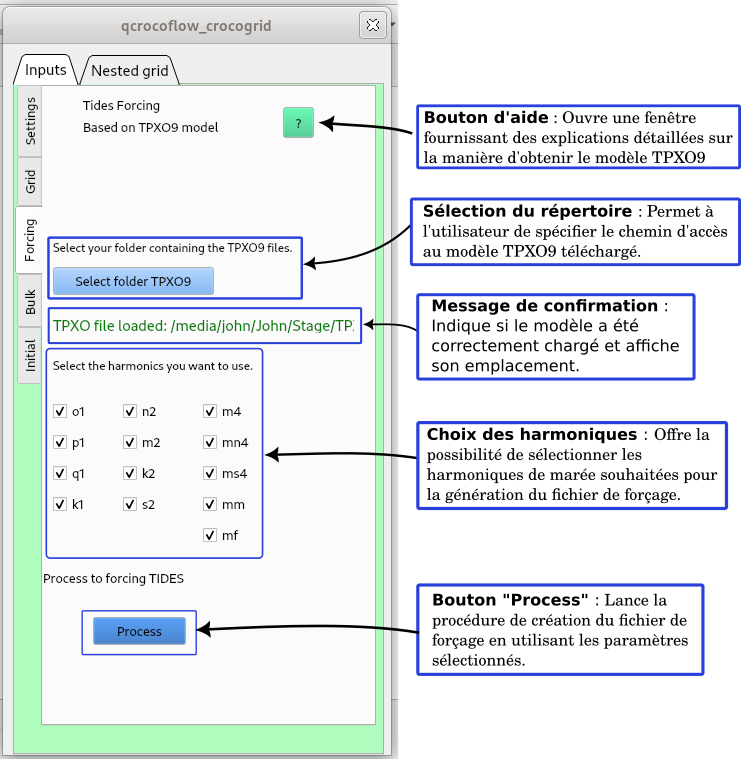
\includegraphics[width=0.8\textwidth]{./IMAGES/Tide/Qcrocotide.png}
	\caption{Capture d'écran de l'interface QCrocoFlow, section "Forcing".}
	\label{fig:qcrocoflow_forcing}
\end{figure}

Après avoir configuré ses préférences, l'utilisateur n'a plus qu'à appuyer sur le bouton \textit{Process} pour initier la création du fichier de forçage. Dans la section suivante, nous détaillerons les étapes techniques sous-jacentes à cette génération.


\subsubsection{Génération du fichier de forçage à partir du modèle TPXO}

La fonction \texttt{TPXO2CROCO} est conçue pour convertir les données du modèle TPXO en un format de forçage adapté à CROCO. Voici une description détaillée de son fonctionnement :

\paragraph{Paramètres d'entrée}
\begin{itemize}
	\item \texttt{t0}: Date initiale choisi par l'utilisateur.
	\item \texttt{ROMSnames}: Liste des composants harmoniques.
	\item \texttt{crocoGRD}: Chemin vers le fichier de grille créer précédemment.
	\item \texttt{fnOut}: Chemin du fichier de sortie.
	\item \texttt{ndays}: Nombre de jours pour lesquels les données doivent être extraites, calculé à partir des dates fournies par l'utilisateur.
	\item \texttt{TPXO\_path}: Chemin vers le répertoire du modèle TPXO.
\end{itemize}


\paragraph{Extraction des données de grille}
Les variables pertinentes, telles que la longitude, la latitude et les masques, sont extraites du fichier de grille CROCO.

\paragraph{Définition des chemins de données TPXO}
Un dictionnaire est créé pour stocker les chemins des différents fichiers de données TPXO, classés par composant harmonique.

\paragraph{Lecture des données TPXO}
Les données TPXO sont lues et interpolées sur la grille CROCO pour chaque composant harmonique sélectionné.

\paragraph{Calcul des corrections nodales}
Les facteurs nodaux sont des coefficients qui varient dans le temps et sont utilisés pour ajuster les amplitudes et les phases des harmoniques de marée. Ces ajustements sont nécessaires car les forces gravitationnelles qui génèrent les marées varient en fonction de la position relative de la Terre, de la Lune et du Soleil. En calculant ces corrections pour une date spécifique, on s'assure que les prédictions des marées sont précises pour cette période donnée.


\paragraph{Interpolation des données TPXO}
Les données TPXO pour chaque composant harmonique sont interpolées sur la grille CROCO. Les amplitudes et les phases sont ensuite converties en paramètres d'ellipse de courant de marée, tels que les axes semi-majeur et semi-mineur, l'excentricité, l'inclinaison et la phase.

\paragraph{Création du fichier netCDF}
Un fichier netCDF est généré pour conserver les données de forçage issues de la transformation. Les données, une fois interpolées, sont enregistrées dans ce format, accompagnées des attributs nécessaires pour garantir leur intégrité et leur compréhension. Ce fichier est sauvegardé dans le même répertoire que la grille de travail, et est nommé en suivant la convention : \textit{"titre du projet"}\_tides.nc.


\paragraph{Message de confirmation}
Une fois le processus terminé, un message est affiché pour informer l'utilisateur que le fichier de forçage a été généré avec succès.\\

En résumé, la fonction \texttt{TPXO2CROCO} a permis d'automatiser le processus de conversion des données TPXO pour les rendre compatibles avec CROCO. Cette automatisation garantit une intégration fluide des effets de marée dans les simulations CROCO, offrant ainsi aux utilisateurs un outil puissant pour leurs études océanographiques.

